\documentclass[tikz,border=2pt]{standalone}
\usepackage{amsmath,amssymb}
\usetikzlibrary{arrows.meta}
\begin{document}
% Annuity-due at annual rate 1 while alive, death at T_x = 2.4 (illustrative):
% m = 1 pays 1 at times 0,1,2; m = 4 pays 1/4 at times 0, 1/4, ..., 9/4 (ten instalments).
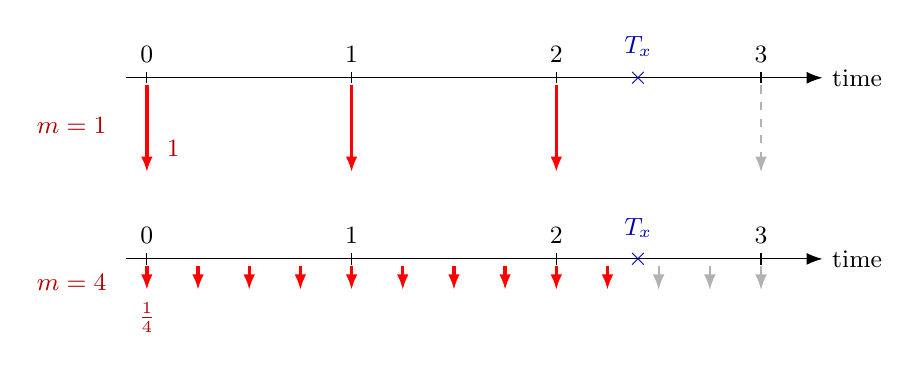
\begin{tikzpicture}[font=\small, >={Latex[length=2mm]}, x=2.6cm, y=1.2cm]
  % m = 1 row
  \begin{scope}
    \draw[->] (-0.1,0) -- (3.3,0) node[right] {time};
    \foreach \k in {0,1,2,3} {\draw (\k,0.06) -- (\k,-0.06); \node[anchor=south] at (\k,0.06) {$\k$};}
    \foreach \k in {0,1,2} \draw[->, red, very thick] (\k,-0.08) -- (\k,-1.0);
    \draw[->, gray!60, thick, dashed] (3,-0.08) -- (3,-1.0);
    \node[red!70!black, anchor=east] at (-0.15,-0.5) {$m=1$};
    \node[red!70!black, anchor=west] at (0.05,-0.75) {$1$};
    \node[blue!70!black, font=\small\bfseries] at (2.4,0) {$\times$};
    \node[blue!70!black, anchor=south] at (2.4,0.12) {$T_x$};
  \end{scope}
  % m = 4 row
  \begin{scope}[yshift=-2.3cm]
    \draw[->] (-0.1,0) -- (3.3,0) node[right] {time};
    \foreach \k in {0,1,2,3} {\draw (\k,0.06) -- (\k,-0.06); \node[anchor=south] at (\k,0.06) {$\k$};}
    \foreach \q in {0,0.25,...,2.26} \draw[->, red, very thick] (\q,-0.08) -- (\q,-0.33);
    \foreach \q in {2.5,2.75,3} \draw[->, gray!60, thick, dashed] (\q,-0.08) -- (\q,-0.33);
    \node[red!70!black, anchor=east] at (-0.15,-0.25) {$m=4$};
    \node[red!70!black, anchor=north] at (0,-0.36) {$\tfrac14$};
    \node[blue!70!black, font=\small\bfseries] at (2.4,0) {$\times$};
    \node[blue!70!black, anchor=south] at (2.4,0.12) {$T_x$};
  \end{scope}
\end{tikzpicture}
\end{document}
